\documentclass[twoside]{article}\usepackage[]{graphicx}\usepackage[]{color}
% maxwidth is the original width if it is less than linewidth
% otherwise use linewidth (to make sure the graphics do not exceed the margin)
\makeatletter
\def\maxwidth{ %
  \ifdim\Gin@nat@width>\linewidth
    \linewidth
  \else
    \Gin@nat@width
  \fi
}
\makeatother

\definecolor{fgcolor}{rgb}{0.345, 0.345, 0.345}
\newcommand{\hlnum}[1]{\textcolor[rgb]{0.686,0.059,0.569}{#1}}%
\newcommand{\hlstr}[1]{\textcolor[rgb]{0.192,0.494,0.8}{#1}}%
\newcommand{\hlcom}[1]{\textcolor[rgb]{0.678,0.584,0.686}{\textit{#1}}}%
\newcommand{\hlopt}[1]{\textcolor[rgb]{0,0,0}{#1}}%
\newcommand{\hlstd}[1]{\textcolor[rgb]{0.345,0.345,0.345}{#1}}%
\newcommand{\hlkwa}[1]{\textcolor[rgb]{0.161,0.373,0.58}{\textbf{#1}}}%
\newcommand{\hlkwb}[1]{\textcolor[rgb]{0.69,0.353,0.396}{#1}}%
\newcommand{\hlkwc}[1]{\textcolor[rgb]{0.333,0.667,0.333}{#1}}%
\newcommand{\hlkwd}[1]{\textcolor[rgb]{0.737,0.353,0.396}{\textbf{#1}}}%
\let\hlipl\hlkwb

\usepackage{framed}
\makeatletter
\newenvironment{kframe}{%
 \def\at@end@of@kframe{}%
 \ifinner\ifhmode%
  \def\at@end@of@kframe{\end{minipage}}%
  \begin{minipage}{\columnwidth}%
 \fi\fi%
 \def\FrameCommand##1{\hskip\@totalleftmargin \hskip-\fboxsep
 \colorbox{shadecolor}{##1}\hskip-\fboxsep
     % There is no \\@totalrightmargin, so:
     \hskip-\linewidth \hskip-\@totalleftmargin \hskip\columnwidth}%
 \MakeFramed {\advance\hsize-\width
   \@totalleftmargin\z@ \linewidth\hsize
   \@setminipage}}%
 {\par\unskip\endMakeFramed%
 \at@end@of@kframe}
\makeatother

\definecolor{shadecolor}{rgb}{.97, .97, .97}
\definecolor{messagecolor}{rgb}{0, 0, 0}
\definecolor{warningcolor}{rgb}{1, 0, 1}
\definecolor{errorcolor}{rgb}{1, 0, 0}
\newenvironment{knitrout}{}{} % an empty environment to be redefined in TeX

\usepackage{alltt}
\usepackage[utf8]{inputenc}
\usepackage[czech]{babel}
\usepackage{fancyhdr}
\usepackage{amsmath}
\usepackage{amsfonts}
\usepackage[paper=a4paper, nomarginpar, foot=1.5cm, top=2.5cm, bottom=2.5cm, left=2.5cm, right=2.5cm]{geometry}
\usepackage{siunitx}

\pagestyle{fancy}
\fancyhead{} % clear all header fields
\fancyhead[RO,LE]{Marek Földi}
\fancyhead[RE,LO]{Úkol 5}
\fancyfoot{} % clear all footer fields
\fancyfoot[LE,RO]{\thepage}

\addto\captioneurosyfilisczech{\renewcommand{\figurename}{Graf. č.}}
\IfFileExists{upquote.sty}{\usepackage{upquote}}{}
\begin{document}





\subsection*{Příklad 1:}
\begin{knitrout}
\definecolor{shadecolor}{rgb}{0.969, 0.969, 0.969}\color{fgcolor}\begin{kframe}
\begin{alltt}
\hlstd{mod1} \hlkwb{<-} \hlkwd{lm}\hlstd{(bota}\hlopt{~}\hlstd{vyska)}
\hlkwd{summary}\hlstd{(mod1)}
\end{alltt}
\begin{verbatim}
## 
## Call:
## lm(formula = bota ~ vyska)
## 
## Residuals:
##     Min      1Q  Median      3Q     Max 
## -3.4310 -0.8385 -0.1015  0.7280  3.9506 
## 
## Coefficients:
##             Estimate Std. Error t value Pr(>|t|)    
## (Intercept) -5.69690    2.20595  -2.583   0.0108 *  
## vyska        0.26590    0.01281  20.764   <2e-16 ***
## ---
## Signif. codes:  0 '***' 0.001 '**' 0.01 '*' 0.05 '.' 0.1 ' ' 1
## 
## Residual standard error: 1.341 on 138 degrees of freedom
## Multiple R-squared:  0.7575,	Adjusted R-squared:  0.7558 
## F-statistic: 431.1 on 1 and 138 DF,  p-value: < 2.2e-16
\end{verbatim}
\end{kframe}
\end{knitrout}
Závislost velikosti boty na výšce je značná. R-squared je skoro 0,76, takže až 76\% velikostí bot lze vysvětlit výškou. Také koeficient pravděpodobnosti je menší než 0,05 a~tudíž velikost boty an výšce závisí.

\newpage
\begin{knitrout}
\definecolor{shadecolor}{rgb}{0.969, 0.969, 0.969}\color{fgcolor}\begin{figure}[h]
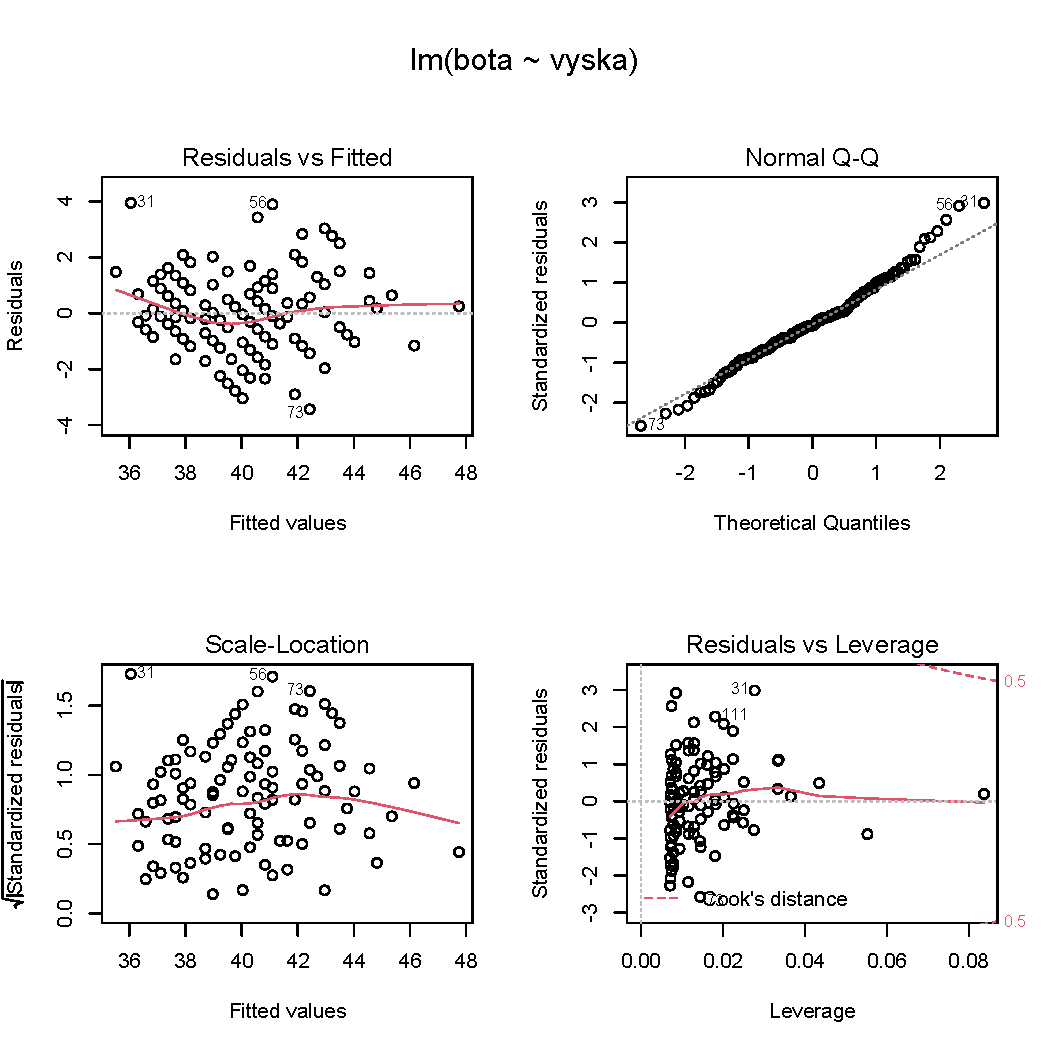
\includegraphics[width=\maxwidth]{figure/plot1-1} \caption[Předpoklady modelu]{Předpoklady modelu}\label{fig:plot1}
\end{figure}


\end{knitrout}
Z~grafů modelu můžeme pozorovat, že model předpoklady splňuje a~nevyskytují se v~něm vzdálená nebo nestandartní pozorovaní, která by model významně ovlivňovala.
\subsection*{Příklad 2:}
\begin{knitrout}
\definecolor{shadecolor}{rgb}{0.969, 0.969, 0.969}\color{fgcolor}\begin{kframe}
\begin{alltt}
\hlstd{mod2} \hlkwb{<-} \hlkwd{lm}\hlstd{(bota}\hlopt{~}\hlstd{vyska} \hlopt{+} \hlstd{pohlavi)}
\hlkwd{summary}\hlstd{(mod2)}
\end{alltt}
\begin{verbatim}
## 
## Call:
## lm(formula = bota ~ vyska + pohlavi)
## 
## Residuals:
##     Min      1Q  Median      3Q     Max 
## -2.4650 -0.8343  0.0011  0.7779  3.3740 
## 
## Coefficients:
##             Estimate Std. Error t value Pr(>|t|)    
## (Intercept)  6.91117    2.62980   2.628  0.00957 ** 
## vyska        0.18927    0.01561  12.123  < 2e-16 ***
## pohlaviM     2.17700    0.31327   6.949 1.36e-10 ***
## ---
## Signif. codes:  0 '***' 0.001 '**' 0.01 '*' 0.05 '.' 0.1 ' ' 1
## 
## Residual standard error: 1.157 on 137 degrees of freedom
## Multiple R-squared:  0.8207,	Adjusted R-squared:  0.8181 
## F-statistic: 313.6 on 2 and 137 DF,  p-value: < 2.2e-16
\end{verbatim}
\begin{alltt}
\hlstd{mod3} \hlkwb{<-} \hlkwd{lm}\hlstd{(bota}\hlopt{~}\hlstd{vyska} \hlopt{*} \hlstd{pohlavi)}
\hlkwd{summary}\hlstd{(mod3)}
\end{alltt}
\begin{verbatim}
## 
## Call:
## lm(formula = bota ~ vyska * pohlavi)
## 
## Residuals:
##     Min      1Q  Median      3Q     Max 
## -2.4526 -0.8308  0.0122  0.7849  3.3365 
## 
## Coefficients:
##                Estimate Std. Error t value Pr(>|t|)    
## (Intercept)     7.47061    3.11537   2.398   0.0178 *  
## vyska           0.18594    0.01850  10.051   <2e-16 ***
## pohlaviM        0.08212    6.21161   0.013   0.9895    
## vyska:pohlaviM  0.01174    0.03476   0.338   0.7361    
## ---
## Signif. codes:  0 '***' 0.001 '**' 0.01 '*' 0.05 '.' 0.1 ' ' 1
## 
## Residual standard error: 1.161 on 136 degrees of freedom
## Multiple R-squared:  0.8209,	Adjusted R-squared:  0.8169 
## F-statistic: 207.7 on 3 and 136 DF,  p-value: < 2.2e-16
\end{verbatim}
\end{kframe}
\end{knitrout}
Z~těchto dvou modelů můžeme usoudit, že pohlaví má na velikost boty vliv. Z~modelu 3 si můžeme všimnout, že pohlaví s~výškou neinteraguje. Tímto modelem můžeme vysvětlit 82 \% velikostí bot. Muž s~výškou 185 cm bude nejspíš mít velikost boty 44,1, vypočteno pomocí: ${6,91117 + 0,18927 \cdot 185 + 2,177 = 44,10312}$

\subsection*{Příklad 3:}
\begin{knitrout}
\definecolor{shadecolor}{rgb}{0.969, 0.969, 0.969}\color{fgcolor}\begin{kframe}
\begin{alltt}
\hlstd{mod4} \hlkwb{<-} \hlkwd{lm}\hlstd{(bota}\hlopt{~}\hlstd{vyska} \hlopt{+} \hlstd{pohlavi} \hlopt{+} \hlstd{vaha} \hlopt{+} \hlstd{zapesti.prave} \hlopt{+} \hlstd{biceps.pravy} \hlopt{+} \hlstd{malicek.pravy)}
\hlkwd{summary}\hlstd{(mod4)}
\end{alltt}
\begin{verbatim}
## 
## Call:
## lm(formula = bota ~ vyska + pohlavi + vaha + zapesti.prave + 
##     biceps.pravy + malicek.pravy)
## 
## Residuals:
##      Min       1Q   Median       3Q      Max 
## -2.09003 -0.78707  0.01282  0.72249  3.13834 
## 
## Coefficients:
##                Estimate Std. Error t value Pr(>|t|)    
## (Intercept)   11.011420   2.940623   3.745  0.00027 ***
## vyska          0.149424   0.018383   8.128 2.86e-13 ***
## pohlaviM       2.049791   0.324922   6.309 4.00e-09 ***
## vaha           0.057738   0.014108   4.092 7.42e-05 ***
## zapesti.prave  0.016343   0.012090   1.352  0.17875    
## biceps.pravy  -0.009336   0.003707  -2.518  0.01300 *  
## malicek.pravy -0.012109   0.014108  -0.858  0.39228    
## ---
## Signif. codes:  0 '***' 0.001 '**' 0.01 '*' 0.05 '.' 0.1 ' ' 1
## 
## Residual standard error: 1.095 on 131 degrees of freedom
##   (2 observations deleted due to missingness)
## Multiple R-squared:  0.845,	Adjusted R-squared:  0.8379 
## F-statistic: 119.1 on 6 and 131 DF,  p-value: < 2.2e-16
\end{verbatim}
\begin{alltt}
\hlstd{mod5} \hlkwb{<-} \hlkwd{lm}\hlstd{(bota}\hlopt{~}\hlstd{vyska} \hlopt{+} \hlstd{pohlavi} \hlopt{+} \hlstd{vaha} \hlopt{+} \hlstd{biceps.pravy)}
\hlkwd{summary}\hlstd{(mod5)}
\end{alltt}
\begin{verbatim}
## 
## Call:
## lm(formula = bota ~ vyska + pohlavi + vaha + biceps.pravy)
## 
## Residuals:
##     Min      1Q  Median      3Q     Max 
## -2.1764 -0.7901 -0.0070  0.7504  3.2272 
## 
## Coefficients:
##               Estimate Std. Error t value Pr(>|t|)    
## (Intercept)  11.753284   2.770387   4.242 4.08e-05 ***
## vyska         0.151738   0.017350   8.745 7.81e-15 ***
## pohlaviM      2.106231   0.306766   6.866 2.19e-10 ***
## vaha          0.056957   0.013632   4.178 5.25e-05 ***
## biceps.pravy -0.007227   0.003479  -2.077   0.0397 *  
## ---
## Signif. codes:  0 '***' 0.001 '**' 0.01 '*' 0.05 '.' 0.1 ' ' 1
## 
## Residual standard error: 1.096 on 135 degrees of freedom
## Multiple R-squared:  0.8416,	Adjusted R-squared:  0.8369 
## F-statistic: 179.3 on 4 and 135 DF,  p-value: < 2.2e-16
\end{verbatim}
\end{kframe}
\end{knitrout}
V~čtvrtém modelu máme všechny navrhované regresory, ale také můžeme pozorovat, že velikost pravého zápěstí a~velikost pravého malíčku jsou nesignifikantní. V~pátém modelu jsou zahrnuty pouze signifikantnější regresory, avšak velikost pravého bicepsu je měně signifikantní a~záporná, to nám může značit, že tento regresor upravuje jiný. Pátý model vysvětluje 83 \% velikostí bot.
\end{document}
